\EnglishSourceFrame{GELFAND-P001425}{1}
\underline{8/II--88.} \underline{Gelfand seminar.}

I. M. G. \underline{Problems.} 1. Calculate
\begin{equation*}
(1)\qquad \det\left\Vert\frac{1}{x_i-y_k}\right\Vert_{i,k=1}^{n}.
\end{equation*}
2. Prove that the Legendre polynomial
\begin{equation*}
\bigl((x^2-1)^n\bigr)^{(n)}
\end{equation*}
has only real zeros.

3. Can a function that is the limit of continuous functions at every point of an interval

a) have discontinuities?

b) have an everywhere dense set of points of discontinuity?

c) be discontinuous everywhere (i.e. at every point)?

4. \textbf{Map conformally onto a disk}

a)\quad
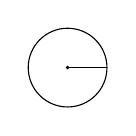
\begin{tikzpicture}[baseline=0cm]
\draw (0,0) circle (0.5);
\fill (0,0) circle (0.025);
\draw (0,0)--(0.5,0);
\end{tikzpicture}
\quad (a disk with a radius removed!)

b)
\begin{center}
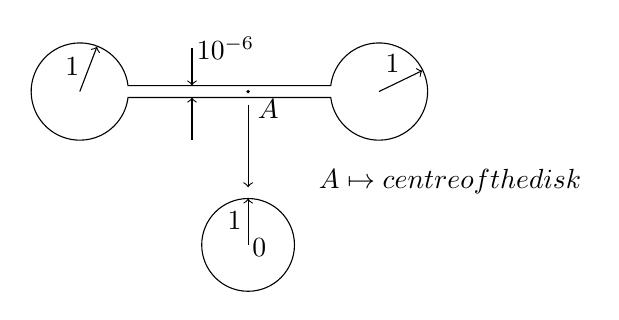
\begin{tikzpicture}[scale=0.95]
\draw (0.645,0.08) arc (7.07:352.93:0.65)
 -- (3.355,-0.08) arc (187.07:532.93:0.65) -- cycle;
\draw[->] (0,0)--(0.23,0.60);
\node at (-0.10,0.33) {$1$};
\draw[->] (4,0)--(4.58,0.28);
\node at (4.18,0.38) {$1$};
\draw[->] (1.5,0.58)--(1.5,0.08);
\draw[->] (1.5,-0.65)--(1.5,-0.08);
\node at (1.95,0.58) {$10^{-6}$};
\fill (2.25,0) circle (0.025);
\node at (2.52,-0.24) {$A$};
\draw[->] (2.25,-0.18)--(2.25,-1.28);
\draw (2.25,-2.05) circle (0.62);
\draw[->] (2.25,-2.05)--(2.25,-1.43);
\node at (2.07,-1.72) {$1$};
\node at (2.40,-2.08) {$0$};
\node at (4.95,-1.20) {$A\mapsto\text{centre of the disk}$};
\end{tikzpicture}
\end{center}

\underline{\textbf{A. Beilinson.}} \qquad
\underline{What should one know about string theory?}

\underline{Conformal field theory.} \qquad (two-dimensional)

Operator expansion.

Connection with representations of natural $\infty$-dimensional Lie algebras.

$W$-algebras, parafermions.

[Crossed out: \EnglishUnclear{GELFAND-P001425}{vertex-cancellation}{Ve\ldots{} / Ver\ldots{} [source beginnings]}]
Algebra of \underline{vertex} operators.
[The beginning of the word ``vertex'' is rewritten over the original strokes.]

Various reductions of representations of $\widehat{SL}_2$ to the Virasoro algebra.

Connection with moduli spaces of algebro-geometric structures.

Explicit formulas for partition functions and
[crossed out: correlation functions; inserted above the line: correlators].

The branching property of characters.

\EnglishSourceFrame{GELFAND-P001426}{unlabelled}
\underline{D. Alekseevsky.} \qquad \underline{$G$-structures}

\underline{Scalar field quantity.}

[Crossed out: Field] --- a function of a point $x\in\mathbb{R}^3$ taking vector values

(e.g. values in $\mathbb{R}$)

\underline{Field quantity:} depends on the coordinate system

\underline{$G$-structure.}

\underline{Definition 1}\quad $G\subset GL(V)$, $V=\mathbb{R}^n$.

[Below $G$:] a linear group.

A $G$-structure [inserted above the line: on $M^n$] is a principal subbundle of the manifold of all
[crossed out: \EnglishUnclear{GELFAND-P001426}{frame-prefix}{ko? [source prefix]}]frames.

[On the right, below ``frames'':] (coframes) --- better to say.

\begin{equation*}
\begin{tikzcd}
M^{(1)} \arrow[r,"GL(V)"] & M
\end{tikzcd}
\end{equation*}
[Below $M^{(1)}$:] the frame bundle (a principal bundle)

\begin{equation*}
\begin{tikzcd}
M^{(1)} \arrow[r,"GL(V)"] & M \\
P \arrow[u,phantom,"\cup" description] \arrow[ur,"G"'] &
\end{tikzcd}
\end{equation*}
$G$ must act transitively on $P$.
\EnglishUnclear{GELFAND-P001426}{transitivity}{transitively on $P$}

Then this is a $G$-structure.

\underline{Examples:} 1) a Riemannian metric is an $O(V)$-structure

2) Let $S$ be a tensor field. When does it define a $G$-structure?

If they are all of the same canonical form

(at $\forall$ point $\exists$ a coframe
[crossed out: \EnglishUnclear{GELFAND-P001426}{tensor-cancellation}{$\theta$ / $\varphi$?}], bringing $S$ to a fixed form)

Then, if $G$ is the automorphism group of the canonical form, $S$ defines a $G$-structure.

3) An affinor defines a $G$-structure if the Jordan form is the same at $\forall$ point

4) An almost complex structure $J$: $G=GL\left(\frac{n}{2},\mathbb{C}\right)$

5) An almost symplectic structure: a 2-form $\sigma$ of maximal rank

(a symplectic structure: $d\sigma=0$)

\underline{Definition 2}\quad A $G$-structure is a principal $G$-bundle
$\pi\colon P\overset{G}{\longrightarrow}M$

$G\subset GL(V)$

equipped with a vector-valued 1-form $\theta\colon TP\to V$,

satisfying the following conditions:

\EnglishSourceFrame{GELFAND-P001427}{2}
a) $G$-equivariance

b) $\operatorname{Ker}\theta=T^vP$ (the vertical space), i.e. $\theta$ is strictly horizontal.

\underline{Equivalence of definitions 1 and 2.}

$p\in P$, $x=\pi p$;
\begin{equation*}
\theta_p\colon T_xM\overset{\simeq}{\longrightarrow}V.
\end{equation*}
[Below $T_xM$, with a bracket and downward arrow:]
\EnglishUnclear{GELFAND-P001427}{quotient-notation}{$(T_pM/T_p^vM)$}.

[On the right:] this is the coframe with which the point $p$ is identified.

[Crossed out: $\theta_p$ on \EnglishUnclear{GELFAND-P001427}{zero-cancellation}{the fibre?} $0$.]

A coframe $\simeq$ an isomorphism $\theta_p\colon T_xM\overset{\simeq}{\longrightarrow}V$.

$\theta$ is called the \underline{displacement form}.

Suppose there is a $G$-structure
\begin{equation*}
(\pi\colon P\overset{G}{\longrightarrow}M;\theta)
\end{equation*}
Consider the bundle of 1-jets of the bundle $\pi$
\begin{equation*}
\pi'\colon P'\to P
\end{equation*}
$x\to p_x$ is a section
\begin{equation*}
p'\colon T_xM\to T_{p_x}P
\end{equation*}
\underline{Definition.} A 1-jet is a map $p'$ inverse to the projection, $p'=j_x^1(p)$
\begin{equation*}
p'=j_x^1(p)\colon
\begin{tikzcd}
T_xM \arrow[r] & T_{p_x}P \arrow[l,bend left=40]
\end{tikzcd}
\end{equation*}
i.e. $\pi_*\circ p'=\mathrm{id}$

\underline{Definition.} A horizontal subspace $H\subset T_pP$
[crossed out: \EnglishUnclear{GELFAND-P001427}{horizontal-cancellation}{illegible}]
is a subspace such that
\begin{equation*}
T_pP=T_p^v\oplus H
\end{equation*}
\underline{Second definition of a 1-jet}

\underline{Elements of $P'$} $=$ \underline{horizontal subspaces}

[Below ``Elements of $P'$'':] ($=$ 1-jets)
\begin{equation*}
p'\in P'\quad\Longleftrightarrow\quad H(p')\text{ is a horizontal subspace}
\end{equation*}
\underline{Relation:}
\begin{equation*}
p'\colon T_xM\to H(p')\subset T_pP
\end{equation*}
\underline{Definition.} [Crossed out: \EnglishUnclear{GELFAND-P001427}{connection-cancellation}{$P'$?}]
$\pi'$ is called the \underline{bundle of connections};

\EnglishSourceFrame{GELFAND-P001428}{unlabelled}
\underline{Space of connections:}\quad $\Gamma(\pi')^G$

(i.e. a connection is a $G$-equivariant section of the bundle $\pi'\colon P'\to P$)

\underline{Connection:}
\begin{equation*}
\begin{aligned}
h\colon P&\to P'\\
p&\mapsto H(p)
\end{aligned}
\end{equation*}
(a $G$-invariant field of horizontal subspaces)

This gives parallel transport (restrict to a curve)

\underline{Torsion function}\qquad (an analogue of a Lie group's structure constants)

There is a vertical parallelism:
\begin{equation*}
\begin{aligned}
i_p\colon\mathfrak g&\overset{\simeq}{\longrightarrow}T_p^vP\\
X&\mapsto X_p:=\left.\frac{d}{dt}(\exp tX)p\right|_{t=0}
\end{aligned}
\end{equation*}
\begin{equation*}
\begin{tikzcd}[column sep=small]
p'\in P'\ \Rightarrow\ T_pP={} & T_p^v \arrow[d,"i_p^{-1}"] & {}\oplus H(p') \\
\pi'(p')=p & \mathfrak g &
\end{tikzcd}
\end{equation*}
[Immediately after the equals sign in the decomposition of $T_pP$, crossed out:
\EnglishUnclear{GELFAND-P001428}{decomposition-cancellation}{illegible}.]

Take the form $\theta_p\colon T_pP\to V$

and put
\begin{equation*}
\theta_{H(p')}=\theta|_{H(p')}\colon H(p')\overset{\simeq}{\longrightarrow}V
\end{equation*}
\underline{Definition.}\quad The \underline{torsion function} is the map
\begin{equation*}
t\colon P'\longrightarrow\operatorname{Hom}(V\wedge V,V)
\end{equation*}
(tensors of type 1,2)
\begin{equation*}
p'\mapsto t_{p'},\qquad
 t_{p'}(\xi,\eta)=d\theta\bigl(\theta_{H(p')}^{-1}\xi,\theta_{H(p')}^{-1}\eta\bigr)
\end{equation*}
\underline{Properties of the torsion function.}

1) $G$-equivariance and $G'=\operatorname{Hom}(V,\mathfrak g)$-equivariance

\EnglishSourceFrame{GELFAND-P001429}{3}
\underline{15/II--88}\qquad \underline{Gelfand's seminar}
(from A.K. Zvonkin's notes)

In I.M.G.'s lectures on quasilinear equations (UMN--59, vol.14, no.2),
\underline{all of thermodynamics} is set out in three pages.

\underline{A concrete geometry problem:} what is the angle between two 2-dimensional subspaces
in a 4-dimensional space?

An angle is an invariant under motion (for lines).

There are two versions: for oriented lines and for unoriented ones.

For planes: how many such invariants are there, and what are they?

\underline{Question:} find all the invariants of two subspaces of a Hilbert space.

[Crossed out: \EnglishUnclear{GELFAND-P001429}{speaker-cancellation}{Zam\ldots{}?}]

\underline{Zamolodchikov, Sasha.}\qquad
\underline{Conformal (2-dimensional) field theory.}

\begin{equation*}
\langle A_1(x_1)A_2(x_2)\ldots A_N(x_N)\rangle,\quad x_i\in\mathbb{R}^2;
\tag{1}
\end{equation*}
--- ``correlation functions''

$\mathcal A\ni A$ --- fields (generally, $\infty$-dimensional)

(1) is an $N$-linear function on the space of fields $\mathcal A$
(and also a function of $(x_1,\ldots,x_N)$).

Let us specify the meaning of the average in (1):
\begin{equation*}
(1)=Z^{-1}\int\mathcal D\varphi\,e^{-S[\varphi]}A_1(x_1)\ldots A_N(x_N),
\tag{2}
\end{equation*}
where $\varphi=\varphi(x)$,
\begin{equation*}
S=\int\sigma\bigl(\varphi(x),\partial\varphi(x)\bigr)\,dx,
\tag{3}
\end{equation*}
\begin{equation*}
Z=\int\mathcal D\varphi\,e^{-S[\varphi]}
\tag{4}
\end{equation*}
[The number (4) is rewritten over \EnglishUnclear{GELFAND-P001429}{equation-number}{3?}.]

\underline{Properties of correlation functions.}

1) ``Algebra of fields''

Suppose the fields form an associative algebra;
[crossed out: \EnglishUnclear{GELFAND-P001429}{algebra-cancellation}{illegible}]
with \EnglishUnclear{GELFAND-P001429}{algebra-ending}{generators [instrumental ending] / generators [genitive ending]} $A_i(x)$.
[Inserted above the line: (with a continuum); the ending of the word ``generators'' is corrected.]

Let $\{A_i\}$ be a basis in $\mathcal A$. Then
\begin{equation*}
A_i(x)A_j(y)=\sum_k c_{ij}^k(x,y)A_k(y)
\end{equation*}
[An arrow to $c_{ij}^k(x,y)$ comes from the caption:] numerical functions of $x,y$

Put
\begin{equation*}
\langle A_k(x)\rangle=a_k(x)
\end{equation*}

\EnglishSourceFrame{GELFAND-P001430}{unlabelled}
(Knowing the functions $c_{ij}^k$ and $a_k$ suffices to calculate the correlation
functions: replace a pair $A_1A_2$ by $\sum c^kA_k$, and so on.)

2) \underline{``Invariance''}

Consider a field $T$ of the form
\begin{equation*}
T^{\mu\nu},\quad\mu,\nu=1,2;\quad T^{\mu\nu}\in\mathcal A.
\end{equation*}
Incidentally,
\begin{equation*}
\frac{\partial}{\partial x^\mu}A_i(x)A_j(y)
=\sum\frac{\partial}{\partial x^\mu}c_{ij}^k(x,y)A_k
\tag{5}
\end{equation*}
\begin{equation*}
\frac{\partial T^{\mu\nu}}{\partial x^\mu}=0
\tag{6}
\end{equation*}
Consider the [crossed out: \EnglishUnclear{GELFAND-P001430}{integral-cancellation}{operator?}] integral
\begin{equation*}
\oint T^{\mu\nu}(x)A(y)\,\varepsilon_{\mu\lambda}\,dx^\lambda
\tag{7}
\end{equation*}
[The index $\lambda$ of $\varepsilon$ is rewritten over
\EnglishUnclear{GELFAND-P001430}{epsilon-first-index}{$\nu$?}.]

[To the right of the integral:]
\begin{center}
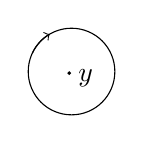
\begin{tikzpicture}
\draw (0,0) circle (0.55);
\draw[->] (155:0.55) arc (155:120:0.55);
\fill (-0.03,-0.02) circle (0.025);
\node at (0.18,-0.08) {$y$};
\end{tikzpicture}
\end{center}
[Callout caption for $\varepsilon$ in (7):]
\begin{equation*}
\varepsilon_{\mu\lambda}=-\varepsilon_{\lambda\mu},\qquad\varepsilon_{12}=1
\end{equation*}
It defines a linear operator on $\mathcal A$.

\underline{Required:} $\exists$ a field $T$ such that this operator equals $\dfrac{\partial}{\partial y}$.

$T^{\mu\nu}:=$ ``energy--momentum tensor''
\begin{equation*}
\oint T^{\mu\nu}(x)A_i(y)\,
\varepsilon_{\mu\nu}
\,dx^\lambda
=\frac{\partial}{\partial y^\nu}A_i(y)
\end{equation*}
\EnglishUnclear{GELFAND-P001430}{epsilon-repeat}{$\varepsilon_{\mu\nu}$}
$1')$\quad $c_{ij}^k(x,y)=c_{ij}^k(x-y)$ --- functions of one variable in $\mathbb R^2$.

3) \underline{``Positivity condition''}

$A\mapsto A^+\in\mathcal A$ is an involution.
\begin{equation*}
A_i^+(x)A_j^+(y)=\sum\overline{c}_{ij}^k(\widetilde x-\widetilde y)A_k^+(y)
\tag{8}
\end{equation*}
\begin{equation*}
x=(x^1,x^2)\quad\Rightarrow\quad\widetilde x=(-x^1,x^2)
\end{equation*}
\underline{Requirement:} the matrix $\langle A_i^+(\widetilde x)A_j(x)\rangle$
is positive definite for every $x$.

\underline{The problem} is to construct substantive examples of all this.

\EnglishSourceFrame{GELFAND-P001431}{4}
Introduce complex coordinates in $\mathbb R^2$
\begin{equation*}
z=x^1+ix^2\qquad ds^2=dz\,d\bar z
\end{equation*}
\begin{equation*}
T^{\nu\mu}=T^{\mu\nu}
\tag{9}
\end{equation*}
\begin{equation*}
\left.\begin{aligned}
T&=T^{zz},\quad\bar T=T^{\bar z\bar z}\\
\Theta&=T^{z\bar z}=0
\end{aligned}\right\}
\quad\begin{gathered}
\text{under these additional conditions}\\
\text{the theory is called ``conformal field theory''}
\end{gathered}
\tag{10}
\end{equation*}
\EnglishUnclear{GELFAND-P001431}{tensor-components}{$T=T^{zz},\ \bar T=T^{\bar z\bar z}$}

[Arrow from below to $\Theta=0$:] Important special case: a massless theory

\underline{Check question:} express $T^{zz}$, $T^{z\bar z}$, $T^{\bar z\bar z}$ in terms of $T^{\mu\nu}$

(this is a linear algebra problem).
\begin{equation*}
\frac{\partial T}{\partial\bar z}=0,\quad
\frac{\partial\bar T}{\partial z}=0
\qquad\text{--- the Cauchy--Riemann equations}
\tag{11}
\end{equation*}
\begin{equation*}
\Updownarrow
\end{equation*}
$T$ is an analytic function of $z$, $T=T(z)$, $\bar T=\bar T(\bar z)$.
\begin{equation*}
T(z)A_i(z_1,\bar z_1)=\sum f_{ij}(z-z_1)A_j(z_1,\bar z_1)
\tag{12}
\end{equation*}
\underline{In electrodynamics:}

$\psi$ --- electron

$A$ --- photon
\begin{equation*}
\{A_i\}=\{\psi,\psi^2,\psi\partial\psi,\ldots,A,A^2,A\psi,\ldots\}
\end{equation*}
$\psi^4$ still exists, but $\psi^5=\psi^6=0$ (since a spinor has only 4 components).

$A$ has all powers.

But, in general, $A^2$ does not exist.

One should take fields at different points, rather than at one point.
\begin{equation*}
\oint\frac{dz}{2\pi i}\,z^{n+1}T(z)A_i(z_1,\bar z_1)
=L_nA_i(z_1,\bar z_1)
\tag{13}
\end{equation*}
[To the right of (13):]
\begin{center}
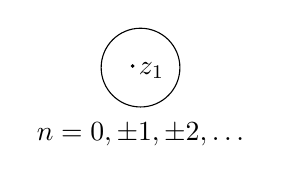
\begin{tikzpicture}
\draw (0,0) circle (0.5);
\fill (-0.10,0.02) circle (0.025);
\node at (0.14,-0.04) {$z_1$};
\node at (0,-0.85) {$n=0,\pm1,\pm2,\ldots$};
\end{tikzpicture}
\end{center}
\begin{equation*}
L_{-1}=\frac{\partial}{\partial z_1}
\end{equation*}
\begin{equation*}
\bar T(\bar z)\to\bar L_n;\quad
\bar L_{-1}=\frac{\partial}{\partial\bar z_1}
\tag{14}
\end{equation*}
$T(z_1)T(z_2)$ is a function of $z_1$, analytic everywhere except at $z_2$;
expand it in a Laurent series.

\EnglishSourceFrame{GELFAND-P001432}{unlabelled}
\begin{equation*}
T(z_1)T(z_2)=\sum_{m=-\infty}^{\infty}(z_1-z_2)^m T_m(z_2),\quad T_m\in\mathcal A
\tag{15}
\end{equation*}
Make an assumption:
\begin{equation*}
(15)=(z_1-z_2)^{-4}T_{-4}+(z-z_2)^{-3}T_{-3}+\ldots
\tag{16}
\end{equation*}
\EnglishUnclear{GELFAND-P001432}{laurent-factor}{$(z-z_2)^{-3}$}

(i.e. the series terminates at the lower end at the $-4$ term).
\begin{equation*}
T_{-1}=\frac{dT}{dz_2}(z_2)
\tag{17}
\end{equation*}
\begin{equation*}
T_{-2}=2T(z_2)\quad\leftarrow\quad
\text{follows from $T$ being a rank-2 tensor}
\tag{18}
\end{equation*}
The most important thing is to determine the most singular terms: $T_{-3}$ and $T_{-4}$.

The positivity condition implies that
\begin{equation*}
T_{-4}\sim\text{identity operator:}\quad T_{-4}=\frac c2,\quad T_{-3}=0
\tag{19}
\end{equation*}
\begin{equation*}
T(z)T(z')=\frac{c}{2(z-z')^4}+\frac{2T(z')}{(z-z')^2}
+\frac{1}{z-z'}T'(z')+\ldots
\tag{20}
\end{equation*}
[Arrow to the ellipsis in (20):] the subsequent terms are of no interest

From this expansion we obtain
\begin{equation*}
\fbox{$[L_n,L_m]=(n-m)L_{n+m}+\frac{c}{12}(n^3-n)\delta_{n+m,0}$}
\tag{21}
\end{equation*}
This is the relation of the \underline{Virasoro algebra} (a central extension of the algebra of vector fields on the circle).

(In ordinary quantum mechanics: the Lie algebra of the group of translations on the line;
$\frac{d}{dx}$ is a small translation --- momentum.)

In general, the energy--momentum tensor comes from coordinate transformations.

In this sense, Sophus Lie invented quantum mechanics: he was the first to replace coordinate transformations by infinitesimal transformations.

(For the Virasoro algebra, the group is the group of diffeomorphisms of the circle.)

Lengths smaller than $10^{-31}$ cm have no meaning --- this assertion no longer depends
[crossed out: \EnglishUnclear{GELFAND-P001432}{lower-cancellation}{on / not}]
on any theory --- it follows from the relations between universal constants.

\EnglishSourceFrame{GELFAND-P001433}{5}
$p$-adic theory has computational advantages: some determinants are best calculated adelically.

But there is something else: physics cannot say anything about nearby points, as well as about distant ones.

[The following paragraph is marked by two vertical lines on the left:]
Everything is known about two-dimensional manifolds, but about three- and four-dimensional ones as little is known as 2000 years ago.

This is a new combinatorics.

How can one conceive of what space is if small distances are forbidden? Imagination is lacking.
(Thickness; discreteness; curvature;\ldots)

[A short horizontal line.]

Conformal invariance: the theory does not change under the substitution
\begin{equation*}
\begin{cases}
z\mapsto z+\varepsilon(z)\\
\bar z\mapsto\bar z+\bar\varepsilon(\bar z)
\end{cases}
\tag{22}
\end{equation*}
Taking $\varepsilon(z)\sim z^{n+1}$ gives the Virasoro algebra.

Let us determine how the average
\begin{equation*}
\langle A_1(x_1)\ldots A_N(x_N)\rangle
=Z^{-1}\int A_1(x_1)\ldots A_N(x_N)e^{-S[\varphi]}\mathcal D\varphi
\tag{23}
\end{equation*}
changes under the substitutions
\begin{equation*}
x^\mu\to x^\mu+\varepsilon^\mu(x)
\tag{24}
\end{equation*}
The variation
\begin{equation*}
\begin{aligned}
\delta\langle A_1(x_1)\ldots A_N(x_N)\rangle
&=\sum_{k=1}^{N}\langle A_1\ldots\delta_\varepsilon A_k\ldots A_N\rangle\\
&\quad+\int\partial_\mu\varepsilon_\nu
\langle T^{\mu\nu}(x)A_1\ldots A_N\rangle\,d^2x=0
\end{aligned}
\tag{25}
\end{equation*}
transfer $\partial_\mu$ to $T^{\mu\nu}$ by integration by parts and use $\partial_\mu T^{\mu\nu}=0$;

integrating over small contours surrounding $x_1,\ldots,x_N$ gives
\begin{equation*}
\delta_\varepsilon A_k(y)=\oint_{c_y}\varepsilon_\nu(x)T^{\lambda\nu}(x)
\varepsilon_{\lambda\mu}\,dx^\mu A_k(y),
\end{equation*}
but
\begin{equation*}
\partial_\mu\varepsilon_\nu+\partial_\nu\varepsilon_\mu=\delta_{\mu\nu}\rho(x);
\end{equation*}
\EnglishUnclear{GELFAND-P001433}{conformal-factor}{$\rho(x)$ / $g(x)$}

$T^{z\bar z}=T^\mu_\mu$ --- the trace; $=0$.
\EnglishUnclear{GELFAND-P001433}{trace-equality}{$T^{z\bar z}=T^\mu_\mu$}

[At the bottom right:]
\begin{center}
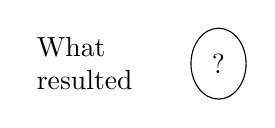
\begin{tikzpicture}
\node[align=left] at (0,0) {What\\resulted};
\draw (1.7,0) ellipse (0.35 and 0.45);
\node at (1.7,0) {?};
\end{tikzpicture}
\end{center}

\EnglishSourceFrame{GELFAND-P001434}{unlabelled}
Fields are classified by representations of the Virasoro algebra.
\begin{equation*}
\left\{\begin{aligned}
L_n\phi_\alpha&=0,\quad n>0;&\qquad\bar L_n\phi_\alpha&=0;\\
L_0\phi_\alpha&=\Delta_\alpha\phi_\alpha;&\qquad
\bar L_0\phi_\alpha&=\bar\Delta_\alpha\phi_\alpha;
\end{aligned}\right.
\tag{26}
\end{equation*}
\begin{equation*}
L_{n_N}\ldots L_{n_1}\phi_\alpha=[\phi_\alpha]
\end{equation*}
\EnglishUnclear{GELFAND-P001434}{descendant-bracket}{$L_{n_N}\ldots L_{n_1}\phi_\alpha=[\phi_\alpha]$}
\begin{equation*}
n_i<0;\quad\Delta_\alpha,\bar\Delta_\alpha\text{ --- two numbers }\geq0
\end{equation*}
\begin{equation*}
\mathcal A=\bigoplus_\alpha[\Phi_\alpha]
\end{equation*}
\begin{equation*}
\mathrm I\in\mathcal A;\qquad\mathrm I\cdot A_i(x)=A_i(x),\quad
\text{for it }\Delta,\bar\Delta=0
\end{equation*}
\begin{equation*}
\begin{gathered}
z\to\lambda z\\
\bar z\to\bar\lambda z
\end{gathered}
\qquad\phi_\alpha\to\lambda^{\Delta_\alpha}\bar\lambda^{\bar\Delta_\alpha}\phi_\alpha,
\end{equation*}
\EnglishUnclear{GELFAND-P001434}{barred-coordinate}{$\bar z\to\bar\lambda z$}
\begin{equation*}
\Delta_\alpha-\bar\Delta_\alpha=S_\alpha\text{ --- the spin of }\phi_\alpha.
\end{equation*}

